\scanpage{7}

% ll. 1–4, 6–7
\mspage{\textcircled{5}}
donc la partition définie par $\deleted{\unsure{\pi_u\{x,\sigma y|\pi_u(x,\sigma y}}\pi_v\varphi_{vu}(\{x,y\})$ ne change pas en remplaçant $x$ par $\sigma(x)$, (ou $y$ par $\sigma(y)$, ou les deux à la fois) donc ne dépend que de $\deleted{\unsure{\widetilde\alpha\rightarrow P_v|\pi_u\varphi}}\alpha=\pi_u(\{x,y\})\in\mathcal P_{\,2,2}(P_u)$ ; enfin, elle ne change pas si on remplace $\alpha$ par $\complement_{P_u}\alpha\dots$

% upper left, first two segments
\figure{\begin{tikzpicture}[x=.78cm,y=.70cm]
\fill (0,0) circle (1.4pt);
\node[below] at (0,-0.01) {$x$};
\node[below] at (0,-0.52) {$\binom{s}{t}$};
\fill (0.85,0) circle (1.4pt);
\node[below] at (0.85,-0.01) {$x'$};
\node[below] at (0.85,-0.52) {$\binom{s'}{t'}$};
\fill (2,0) circle (1.4pt);
\node[below] at (2,-0.01) {$y$};
\node[below] at (2,-0.52) {$\binom{s}{t}$};
\fill (2.85,0) circle (1.4pt);
\node[below] at (2.85,-0.01) {$y'$};
\node[below] at (2.85,-0.52) {$\binom{s'}{t'}$};
\draw[very thick] (0,0)--(.85,0) (2,0)--(2.85,0);
\end{tikzpicture}}

% upper left, second two segments
\figure{\begin{tikzpicture}[x=.78cm,y=.70cm]
\fill (0,0) circle (1.4pt);
\node[above] at (0,0) {$\zeta$};
\node[below] at (0,-0.12) {$\binom{s}{t'}$};
\fill (0.85,0) circle (1.4pt);
\node[above] at (0.85,0) {$\zeta'$};
\node[below] at (0.85,-0.12) {$\binom{s'}{t}$};
\fill (2,0) circle (1.4pt);
\node[above] at (2,0) {$\eta$};
\node[below] at (2,-0.12) {$\binom{s}{t'}$};
\fill (2.85,0) circle (1.4pt);
\node[above] at (2.85,0) {$\eta'$};
\node[below] at (2.85,-0.12) {$\binom{s'}{t}$};
\draw[very thick] (0,0)--(.85,0) (2,0)--(2.85,0);
\end{tikzpicture}}

% upper centre, joined pairs
\figure{\begin{tikzpicture}[x=.78cm,y=.70cm]
\fill (0,0) circle (1.4pt);
\node[below] at (0,-0.01) {$s$};
\node[below] at (0,-0.52) {$\binom{x}{y}$};
\fill (0.85,0) circle (1.4pt);
\node[below] at (0.85,-0.01) {$s'$};
\node[below] at (0.85,-0.52) {$\binom{x'}{y'}$};
\fill (2,0) circle (1.4pt);
\node[below] at (2,-0.01) {$t$};
\node[below] at (2,-0.52) {$\binom{x}{y}$};
\fill (2.85,0) circle (1.4pt);
\node[below] at (2.85,-0.01) {$t'$};
\node[below] at (2.85,-0.52) {$\binom{x'}{y'}$};
\draw[very thick] (0,0)--(.85,0) (2,0)--(2.85,0);
\draw (0,.19)--(.98,1.13)--(1.96,.18) (.85,.2)--(1.83,1.25)--(2.82,.18);
\end{tikzpicture}}

% upper centre right, cancelled pairs
\figure{\begin{tikzpicture}[x=.78cm,y=.70cm]
\fill (0,0) circle (1.4pt);
\node[below] at (0,-0.01) {$\unsure{u}$};
\node[below] at (0,-0.52) {$\binom{x}{\unsure{y''|y'}}$};
\fill (0.85,0) circle (1.4pt);
\node[below] at (0.85,-0.01) {$u'$};
\node[below] at (0.85,-0.52) {$\binom{x'}{y}$};
\fill (2,0) circle (1.4pt);
\node[below] at (2,-0.01) {$v$};
\node[below] at (2,-0.52) {$\binom{x}{y'}$};
\fill (2.85,0) circle (1.4pt);
\node[below] at (2.85,-0.01) {$v'$};
\node[below] at (2.85,-0.52) {$\binom{x'}{y}$};
\draw[very thick] (0,0)--(.85,0) (2,0)--(2.85,0);
\draw (0,.19)--(.98,1.13)--(1.96,.18) (.85,.2)--(1.83,1.25)--(2.82,.18);
\draw (0,.6) .. controls (0,-2.3) and (.1,1.3) .. (1.2,1.1) -- (.2,-1.7) -- (2.25,1.15) -- (.8,-1.75) -- (2.65,.75) .. controls (2,-1.9) and (1.9,.65) .. (3.06,.23) -- (2.68,-1.5) -- (.25,-1.48);
\end{tikzpicture}}

% ll. 8–10
\uline{\deleted{Corollaire}\inserted{Lemme} 6} $c_{wv}c_{vu}=c_{wu}$ --- donc les $c_{vu}$ etc définissent un syst. transitif d'iso entre les $\Pi_{22}(P_u),\Pi_{22}(P_v),\Pi_{22}(P_w)$

% ll. 11–13, crossed diagonally
\deleted{Soit $\{s,t\}=\unsure{\tau_{vu}|c_{vu}}\{x,y\}$ \inserted{$(x,y\in E(u)^*$ non liés)}. Soit $\zeta\in E(w)^*$ lié à $x$ et $s$, (lemme 5 a)), $\eta\in E(w)^*$ lié à $y,t$.}

% left of ll. 10–13
\figure{\begin{tikzpicture}[scale=.85]
\draw (0,.28)--(2.1,0)--(1.98,2.2);
\node[left] at (0,.22) {$x$}; \node[below] at (.25,.18) {$y$};
\node[right] at (2.1,0) {$s\quad t$};
\fill (1.98,2.67) circle(.8pt) node[above] {$w$};
\fill (.92,1.36) circle(.8pt) node[above] {$u$};
\fill (2.64,1.39) circle(.8pt) node[right] {$v$};
\end{tikzpicture}}

% l. 14
Cela \deleted{\unsure{résulte du|résulte}}\inserted{est inclus dans le} résultat plus précis

% ll. 15–16
\[
\begin{aligned}
\text{\uline{Corollaire}}\qquad
\widetilde\varphi_{wv}\widetilde\varphi_{vu}(\widetilde\alpha)&=\sigma(\widetilde\varphi_{wu}(\widetilde\alpha))\qquad\text{i.e.}\\
\widetilde\varphi_{wv}\widetilde\varphi_{vu}&=\sigma\widetilde\varphi_{wu}
\end{aligned}
\]

% ll. 17–19
\[
\begin{aligned}
\text{i.e.}\quad x,y\in E(u)^*&\quad x,y\text{ liés à }s,t\\
s,t\in E(v)^*&\quad s,t\text{ liés à }p,q\\
\{p,q\}\in E(w)^*&\quad\Longrightarrow xy\text{ liés à }\sigma p,\sigma q
\end{aligned}
\]

% lower left, first polyhedron
\figure{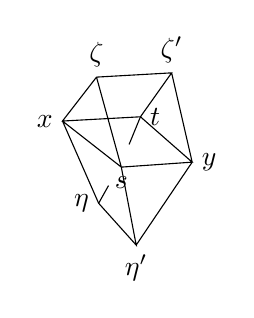
\begin{tikzpicture}[scale=.9]
\coordinate (x) at (0,1.2);\coordinate (t) at (1.1,1.26);\coordinate (y) at (1.83,.62);\coordinate (s) at (.83,.55);
\coordinate (z) at (.48,1.82);\coordinate (zz) at (1.54,1.88);\coordinate (h) at (.51,.04);\coordinate (hh) at (1.04,-.55);
\draw (x)--(z)--(zz)--(t)--cycle (x)--(s)--(y)--(t) (z)--(s)--(hh)--(h)--(x) (y)--(hh) (zz)--(y);
\draw (h)--(.65,.29) (t)--(.94,.87);
\node[left] at (x) {$x$}; \node[right] at (t) {$t$}; \node[right] at (y) {$y$}; \node[below] at (s) {$s$};
\node[above] at (z) {$\zeta$}; \node[above] at (zz) {$\zeta'$}; \node[left] at (h) {$\eta$}; \node[below] at (hh) {$\eta'$};
\end{tikzpicture}}

% lower left below first drawing, struck through
\figure{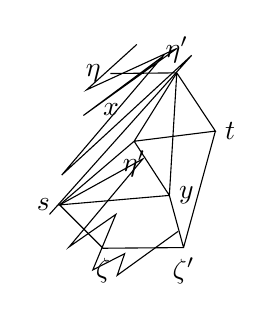
\begin{tikzpicture}[scale=.86]
\coordinate (a) at (.75,1.8);\coordinate (b) at (1.73,1.81);\coordinate (c) at (2.3,.95);\coordinate (d) at (1.62,0);
\coordinate (e) at (0,-.14);\coordinate (f) at (.64,-.78);\coordinate (g) at (1.83,-.77);\coordinate (h) at (1.10,.8);
\draw (a)--(b)--(c)--(h)--(e)--(d)--(b) (e)--(f)--(g)--(c) (g)--(d)--(h)--(b);
\node[left] at (e) {$s$};\node[right] at (c) {$t$};\node[left] at (a) {$\eta$};\node[above] at (b) {$\unsure{\eta'}$};
\node[above] at (.76,1.03) {$x$};\node[below] at (h) {$\eta'$};\node[right] at (d) {$y$};\node[below] at (f) {$\zeta$};\node[below] at (g) {$\zeta'$};
\draw (-.15,-.28)--(1.95,2.07)--(.03,.3)--(1.52,2.05)--(.35,1.18)--(1.73,2.17)--(.4,1.56)--(1.14,2.23)
 (0,-.14)--(1.23,.54)--(.14,-.76)--(.83,-.28)--(.49,-1.10)--(.96,-.86)--(.85,-1.18)--(1.75,-.53);
\end{tikzpicture}}

% ll. 20–23
Prouvons d'abord le lemme 6. Comme \unsure{ds|dans} lemme 5, complétons les triangles

% ll. 22–23
\[
\begin{aligned}
(x,s,\zeta),\ (y,t,\zeta')&\quad(\zeta,\zeta'\in E(w)^*\text{ sont liés})\\
(x,t,\eta),\ (y,s,\eta')&\quad(\eta,\eta'\in E(w)^*\text{ sont liés})
\end{aligned}
\]

% ll. 24–26
Alors $\zeta$ lié à $s$, \uline{non à $t$} (sinon $(\zeta,t)$ appartiendrait à 2 triangles de sommets $x,\zeta'$) de $=$ $\eta$ lié à $t$, non à $s$, donc cela montre que

% l. 27
\[
\{\pi_w(\{\zeta,\eta\}),\complement_{P_w}\pi_w(\{\zeta,\eta\})\}
=\unsure{\widetilde\varphi_{wv}|c_{wv}}(\pi_{\unsure{w|v}}\{s,t\},\complement\pi_w(\{s,t\})),
\]

% ll. 28–29
Mais aussi $\zeta$ lié à $x$, non à $y$, $\eta$ lié à $x$, non à $y$ donc $\{\pi_w(\{\zeta,\eta\}),\complement\pi_w(\{\zeta,\eta\})\}=c_{wu}'(\pi_u(\{x,y\}),\complement\pi_u(\{x,y\}))$
% archive sheet number: 6
